%<dscrpt>Somme sur un triangle : un pas vers l'exponentielle.</dscrpt>
\begin{figure}[htp]
 \centering
 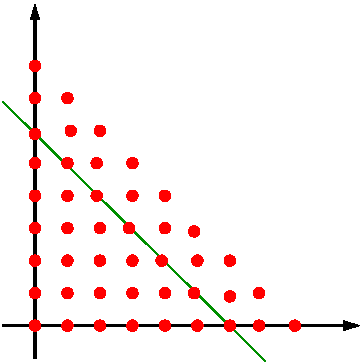
\includegraphics{Esomm1_1.pdf}
 \caption{$\mathcal T$ et un $\mathcal{D}_p$}
 \label{fig:Esomm1_1}
\end{figure}

Soit $n$ un entier naturel non nul. On définit des parties $\mathcal{T}$ et $\mathcal{D}_p$ pour $p\in\left\lbrace 0,1,\cdots , n\right\rbrace$
\begin{displaymath}
 \forall (i,j)\in \N^2 :
\left. 
\begin{aligned}
 (i,j) \in \mathcal T &\Leftrightarrow i + j \leq n \\
 (i,j) \in \mathcal{D}_p &\Leftrightarrow i + j =p 
\end{aligned}
\right. 
\end{displaymath}
\begin{enumerate}
 \item Rappeler sans démonstration la formule donnant un coefficient du binôme uniquement à l'aide de factorielles.
 \item Soit $x$ et $y$ deux nombres complexes, en utilisant $\mathcal{T}$ et $\mathcal{D}_p$, donner une autre expression de la somme
\begin{displaymath}
 S = \sum_{(i,j)\in \mathcal T}\frac{x^i}{i!}\frac{y^j}{j!}
\end{displaymath}

\end{enumerate}
